%% LyX 2.3.6.1 created this file.  For more info, see http://www.lyx.org/.
%% Do not edit unless you really know what you are doing.
\documentclass[11pt,oneside,czech,american]{book}
\usepackage[T1]{fontenc}
\usepackage[utf8]{inputenc}
\usepackage[a4paper]{geometry}
\geometry{verbose,tmargin=4cm,bmargin=3cm,lmargin=3cm,rmargin=2cm,headheight=0.8cm,headsep=1cm,footskip=0.5cm}
\pagestyle{headings}
\setcounter{secnumdepth}{3}
\usepackage{url}
\usepackage{amsmath}
\usepackage{amsthm}
\usepackage{amssymb}
\usepackage{graphicx}
\usepackage{setspace}
\usepackage{enumitem}
\makeatletter

\newtheorem{theorem}{Theorem}
\theoremstyle{definition}
\newtheorem{definition}{Definition}

%%%%%%%%%%%%%%%%%%%%%%%%%%%%%% Textclass specific LaTeX commands.
\newenvironment{lyxlist}[1]
	{\begin{list}{}
		{\settowidth{\labelwidth}{#1}
		 \setlength{\leftmargin}{\labelwidth}
		 \addtolength{\leftmargin}{\labelsep}
		 \renewcommand{\makelabel}[1]{##1\hfil}}}
	{\end{list}}

%%%%%%%%%%%%%%%%%%%%%%%%%%%%%% User specified LaTeX commands.
%% Font setup: please leave the LyX font settings all set to 'default'
%% if you want to use any of these packages:

%% Use Times New Roman font for text and Belleek font for math
%% Please make sure that the 'esint' package is turned off in the
%% 'Math options' page.
\usepackage[varg]{txfonts}

%% Use Utopia text with Fourier-GUTenberg math
%\usepackage{fourier}

%% Bitstream Charter text with Math Design math
%\usepackage[charter]{mathdesign}

%%---------------------------------------------------------------------

%% Make the multiline figure/table captions indent so that the second
%% line "hangs" right below the first one.
%\usepackage[format=hang]{caption}

%% Indent even the first paragraph in each section
\usepackage{indentfirst}

%%---------------------------------------------------------------------

%% Disable page numbers in the TOC. LOF, LOT (TOC automatically
%% adds \thispagestyle{chapter} if not overriden
%\addtocontents{toc}{\protect\thispagestyle{empty}}
%\addtocontents{lof}{\protect\thispagestyle{empty}}
%\addtocontents{lot}{\protect\thispagestyle{empty}}

%% Shifts the top line of the TOC (not the title) 1cm upwards 
%% so that the whole TOC fits on 1 page. Additional page size
%% adjustment is performed at the point where the TOC
%% is inserted.
%\addtocontents{toc}{\protect\vspace{-1cm}}

%%---------------------------------------------------------------------

% completely avoid orphans (first lines of a new paragraph on the bottom of a page)
\clubpenalty=9500

% completely avoid widows (last lines of paragraph on a new page)
\widowpenalty=9500

% disable hyphenation of acronyms
\hyphenation{CDFA HARDI HiPPIES IKEM InterTrack MEGIDDO MIMD MPFA DICOM ASCLEPIOS MedInria}

%%---------------------------------------------------------------------

%% Print out all vectors in bold type instead of printing an arrow above them
\renewcommand{\vec}[1]{\boldsymbol{#1}}

% Replace standard \cite by the parenthetical variant \citep
%\renewcommand{\cite}{\citep}

\makeatother

\usepackage{babel}
\begin{document}
\def\documentdate{August 2, 2023}

%%\def\documentdate{\today}

\pagestyle{empty}
{\centering

\noindent %
\begin{minipage}[c]{3cm}%
\noindent \begin{center}

\includegraphics[width=3cm,height=3cm,keepaspectratio]{Images/TITLE/cvut}
\par\end{center}%
\end{minipage}%
\begin{minipage}[c]{0.6\linewidth}%
\begin{center}
\textsc{\large{}Czech Technical University in Prague}{\large{}}\\
{\large{}Faculty of Nuclear Sciences and Physical Engineering}
\par\end{center}%
\end{minipage}%
\begin{minipage}[c]{3cm}%
\noindent \begin{center}
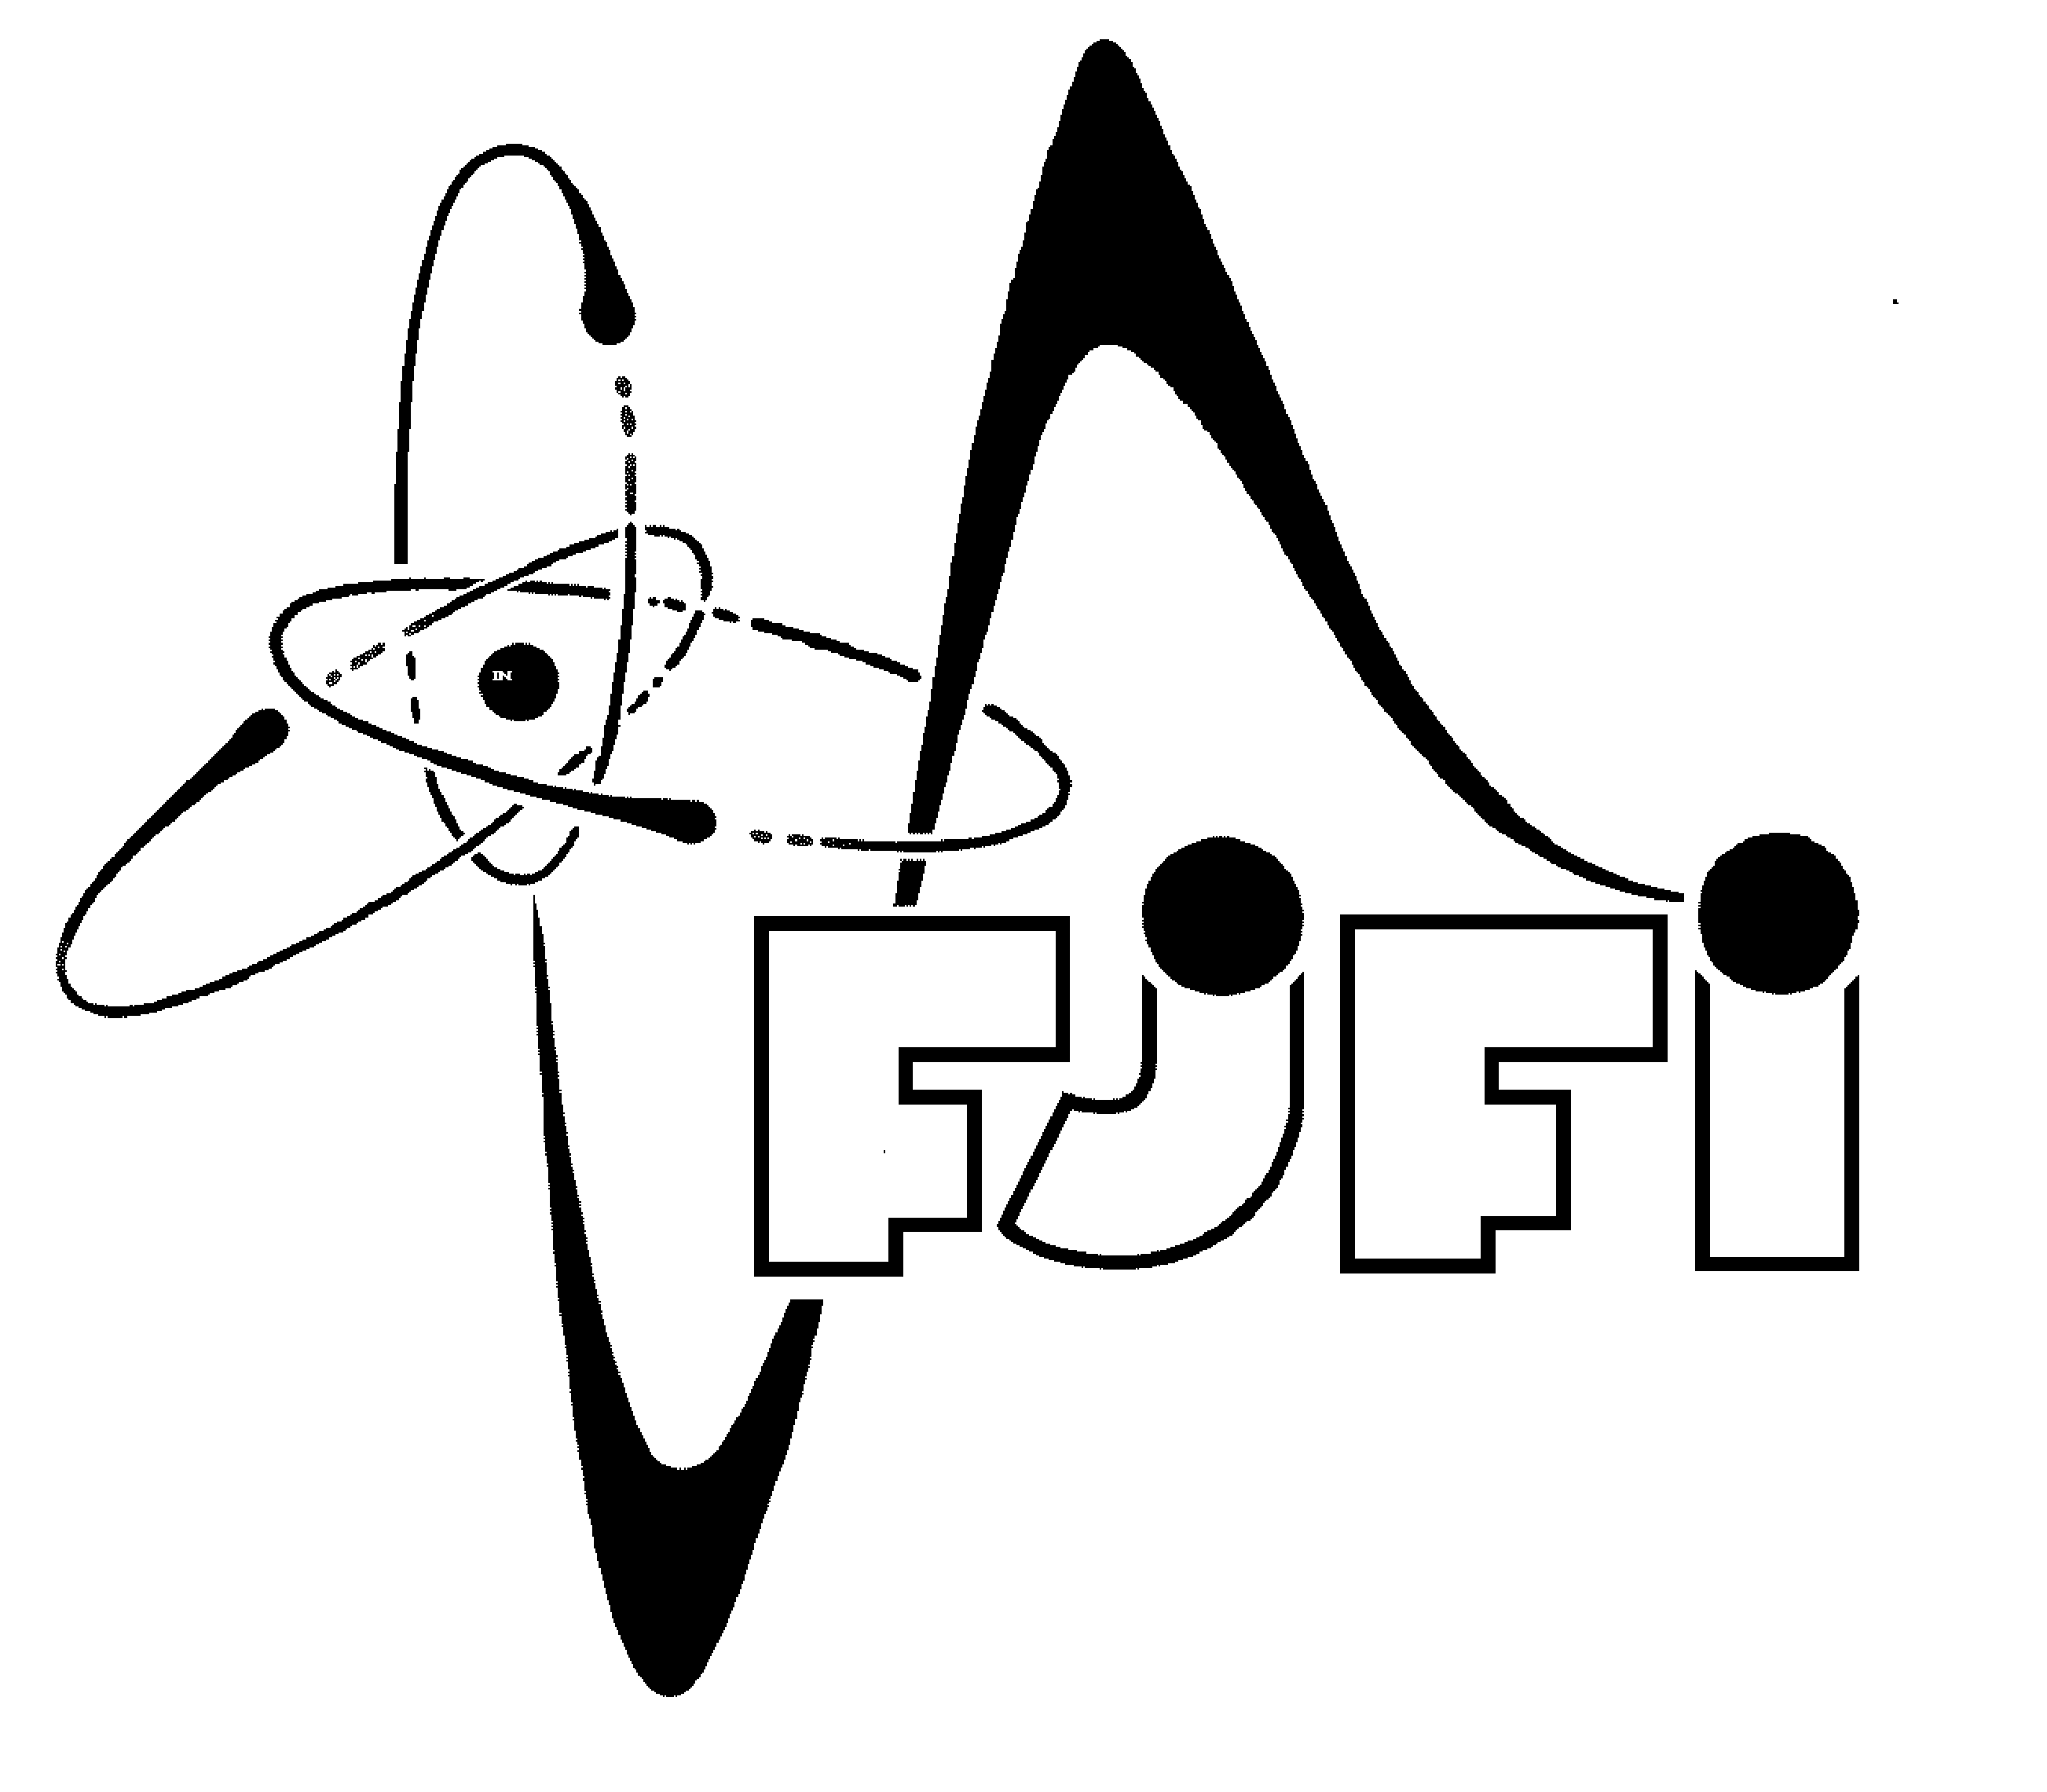
\includegraphics[width=3cm,height=3cm,keepaspectratio]{Images/TITLE/fjfi}
\par\end{center}%
\end{minipage}

\vspace{3cm}

\textbf{\huge{}Classification of Ultrasound Signals Using Neural Networks}{\huge\par}

\vspace{1cm}

\selectlanguage{czech}%
\textbf{\huge{}Klasifikace ultrazvukových signálů pomocí neuronových sítí}{\huge\par}

\selectlanguage{american}%
\vspace{2cm}

{\large{}Bachelor's Degree Project}{\large\par}

}

\vfill{}

\begin{lyxlist}{MMMMMMMMM}
\begin{singlespace}
\item [{Author:}] \textbf{Petr Vojtášek}
\item [{Supervisor:}] \textbf{Ing. Martin Kovanda}
\item [{Consultant:}] \textbf{Ing. Milan Chlada, Ph.D.}
\end{singlespace}
\item [{Language~advisor:}] \textbf{Mgr. Jméno Učitelky Angličtiny}
\begin{singlespace}
\item [{Academic~year:}] 2023/2024
\end{singlespace}
\end{lyxlist}
\newpage{}

~

\vfill{}

\begin{center}
- Zadání práce -
\par\end{center}

\vfill{}

~\newpage{}

~

\vfill{}

\begin{center}
- Zadání práce (zadní strana) -
\par\end{center}

\vfill{}

~\newpage{}

\noindent \emph{\Large{}Acknowledgment:}{\Large\par}

\noindent I would like to thank Ing. Martin Kovanda
for his expert guidance.

\vfill

\noindent \emph{\Large{}Author's declaration:}{\Large\par}

\noindent I declare that this Bachelor's Degree Project is entirely
my own work and I have listed all the used sources in the bibliography.

\bigskip{}

\noindent Prague, \documentdate\hfill{}Jméno Autora

\vspace{2cm}

\newpage{}

\selectlanguage{czech}%
\begin{onehalfspace}
\noindent \emph{Název práce:}

\noindent \textbf{Název práce}
\end{onehalfspace}

\bigskip{}

\noindent \emph{Autor:} Jméno Autora

\bigskip{}

\noindent \emph{Obor:} Celý název oboru (nikoliv zkratka)\bigskip{}

\noindent \emph{Zaměření:} Celý název zaměření (Pokud obor neobsahuje
zaměření, tuto řádku odstranit.)

\bigskip{}

\noindent \emph{Druh práce:} Bakalářská práce

\bigskip{}

\noindent \emph{Vedoucí práce:} prof. Ing. Jméno Školitele, DrSc.,
pracoviště školitele (název instituce, fakulty, katedry...)

\bigskip{}

\noindent \emph{Konzultant:} doc. RNDr. Jméno Konzultanta, CSc., pracoviště
konzultanta. Pouze pokud konzultant byl jmenován.

\bigskip{}

\noindent \emph{Abstrakt:} Abstrakt max. na 10 řádků. Abstrakt max.
na 10 řádků. Abstrakt max. na 10 řádků. Abstrakt max. na 10 řádků.
Abstrakt max. na 10 řádků. Abstrakt max. na 10 řádků. Abstrakt max.
na 10 řádků. Abstrakt max. na 10 řádků. Abstrakt max. na 10 řádků.
Abstrakt max. na 10 řádků. Abstrakt max. na 10 řádků. Abstrakt max.
na 10 řádků. Abstrakt max. na 10 řádků. Abstrakt max. na 10 řádků.
Abstrakt max. na 10 řádků. Abstrakt max. na 10 řádků. Abstrakt max.
na 10 řádků. Abstrakt max. na 10 řádků. Abstrakt max. na 10 řádků.
Abstrakt max. na 10 řádků. Abstrakt max. na 10 řádků. Abstrakt max.
na 10 řádků. Abstrakt max. na 10 řádků. Abstrakt max. na 10 řádků.
Abstrakt max. na 10 řádků. Abstrakt max. na 10 řádků. Abstrakt max.
na 10 řádků. Abstrakt max. na 10 řádků. Abstrakt max. na 10 řádků. 

\bigskip{}

\noindent \emph{Klíčová slova:} klíčová slova (nebo výrazy) seřazená
podle abecedy a oddělená čárkou

\selectlanguage{american}%
\vfill{}
~

\begin{onehalfspace}
\noindent \emph{Title:}

\noindent \textbf{Title of the Work}
\end{onehalfspace}

\bigskip{}

\noindent \emph{Author:} Author's Name

\bigskip{}

\noindent \emph{Abstract:} Max. 10 lines of English abstract text.
Max. 10 lines of English abstract text. Max. 10 lines of English abstract
text. Max. 10 lines of English abstract text. Max. 10 lines of English
abstract text. Max. 10 lines of English abstract text. Max. 10 lines
of English abstract text. Max. 10 lines of English abstract text.
Max. 10 lines of English abstract text. Max. 10 lines of English abstract
text. Max. 10 lines of English abstract text. Max. 10 lines of English
abstract text. Max. 10 lines of English abstract text. Max. 10 lines
of English abstract text. Max. 10 lines of English abstract text.
Max. 10 lines of English abstract text. Max. 10 lines of English abstract
text. Max. 10 lines of English abstract text. Max. 10 lines of English
abstract text. Max. 10 lines of English abstract text. Max. 10 lines
of English abstract text. Max. 10 lines of English abstract text.
Max. 10 lines of English abstract text. Max. 10 lines of English abstract
text. Max. 10 lines of English abstract text.

\bigskip{}

\noindent \emph{Key words:} keywords in alphabetical order separated
by commas

\newpage{}

\pagestyle{plain}

\tableofcontents{}

\newpage{}

\chapter*{Introduction}

\addcontentsline{toc}{chapter}{Introduction}

Paragraphs of the Introduction\ldots{}

\chapter{Neural networks}

jJjjajaj \cite{Goodfellow-conv} jkajjasj






\section{Feed forward networks}
The building block for deep learning is feed-forward neural networks. They are also the least complex architectures, and all the basic principles such as the learning process are easiest to explain using the example of a feed-forward network. The main goal of a neural network is to approximate a function $f$ which, explicitly for classification, maps an input $\Vec{x}$ to a vector of categories $\Vec{y}$.
\par The Simplest way to represent a feed-forward network is as directed acyclic graphs 
\ref{FF_graph}, where each node represents a neuron and each edge represents a weight that is multiplied by the output from the initial node. Nodes are aligned in layers and except the initial layer, all neurons in each layer are fully connected to neurons in the previous layer. Between the input layer and the output layer are hidden layers. The number of hidden layers is associated with the depth of the network, hence the name deep learning.

\begin{figure}[h]
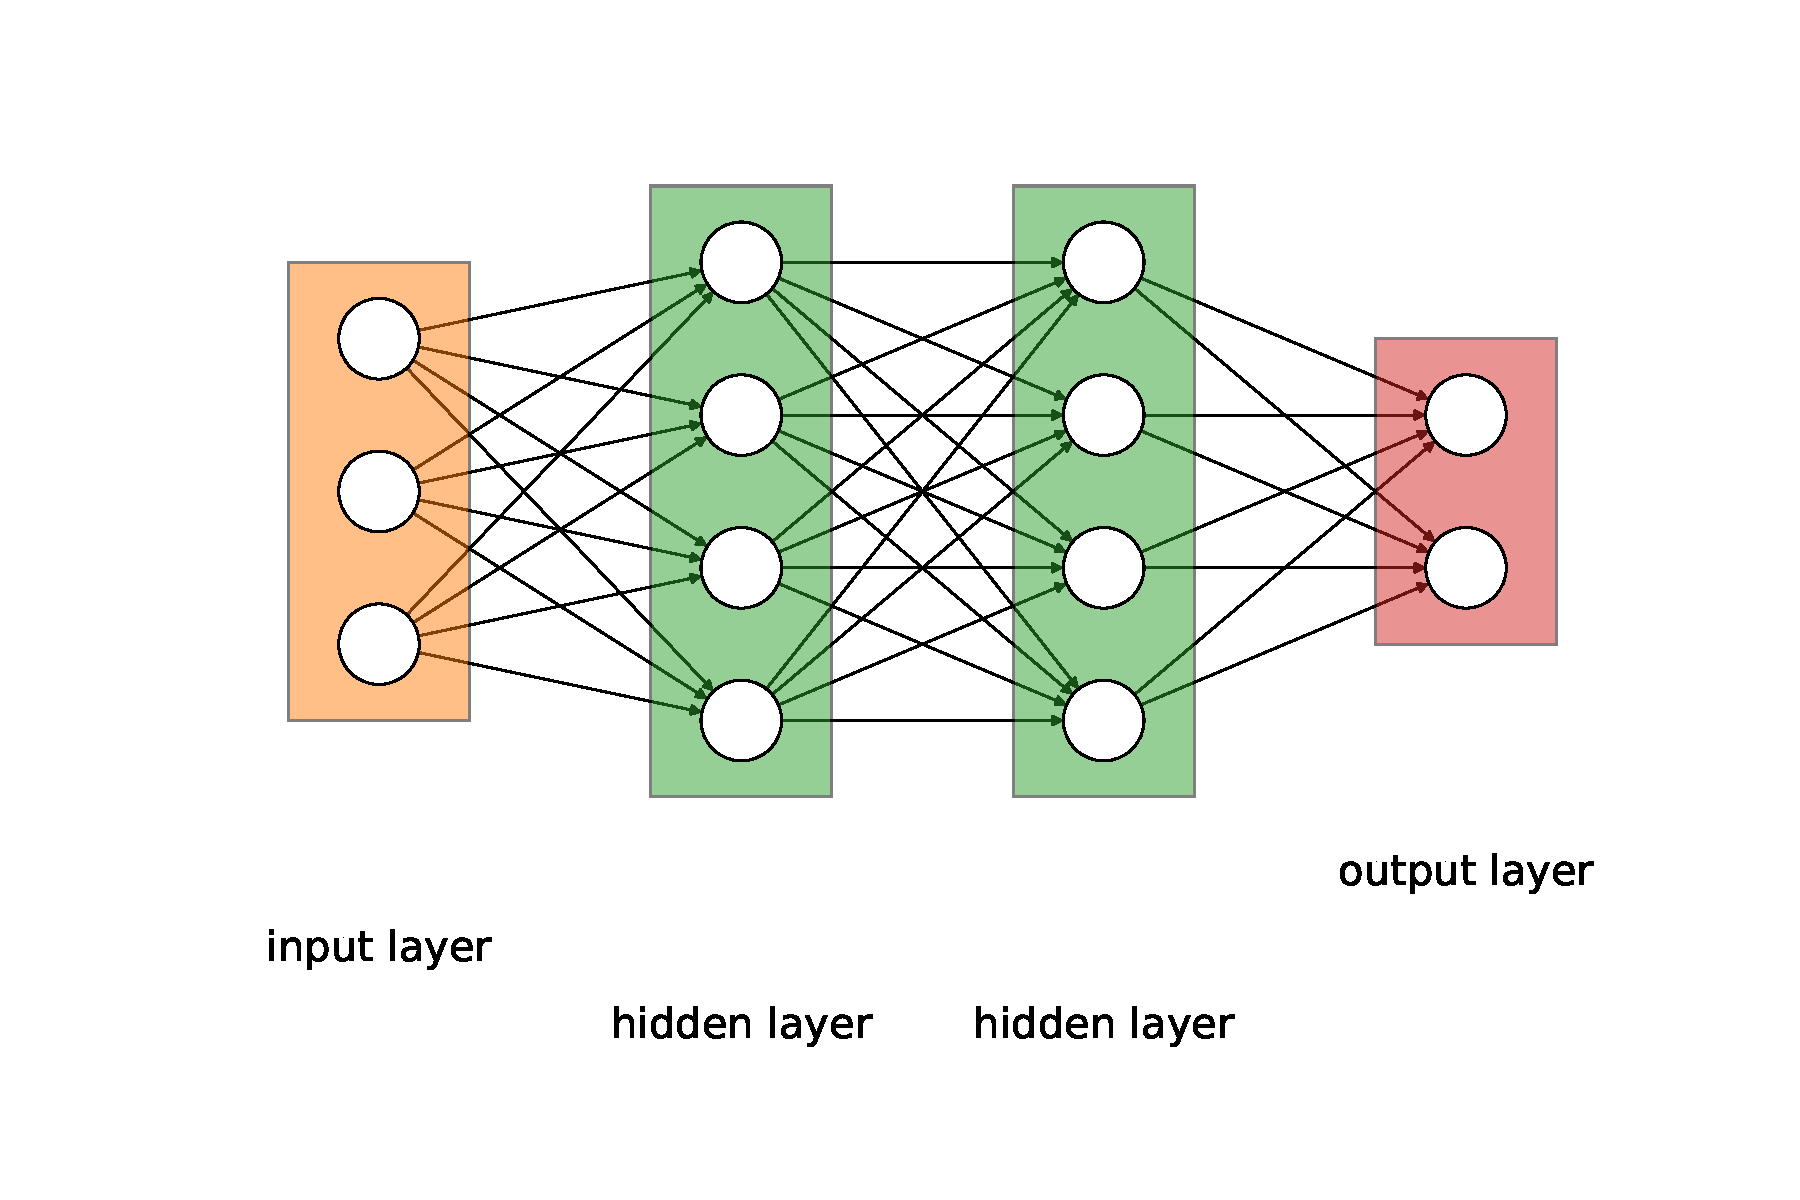
\includegraphics[width=0.7\textwidth]{Images/ff_graph.pdf}
\label{FF_graph}
\centering
\caption{Feed forward neural network as directed acyclic graph. Will be better in the future}
\end{figure}

In each neuron, a weighted sum of all inputs from the previous layer is calculated with the addition of a constant called bias.
\par Weighted sum for $i$-th layer: 

\begin{equation}
    \Vec{z^{i}} = \Vec{W^{i}}\Vec{y^{i-1}} + \Vec{b^i}
    \label{weighted sum}
\end{equation}

Where $y^{i-1}$ is the output of the $(i-1)$-th layer and $b_i$ is the bias. For the first layer, we set $\Vec{y^0} = \Vec{x}$, where $\Vec{c}$ is the input vector. A non-linear activation function $f$ is then applied to this weighted sum.

\begin{equation}
    \Vec{y^i} = f(\Vec{z^i})
\end{equation}

These two equations can describe what a feed-forward network represents. In summary, a feed-forward network is just a composition of multiple nonlinear transformations.










\section{Activation functions}
\label{sec: Activation functions}
The composition of multiple linear transformations remains linear. The non-linearity is assured by the output function called activation. The choice of activation function affects the performance of our model. 
\subsection{Properties of most used activation functions}
    \paragraph{Rectified linear unit}
    Currently the most widely-used activation function because of its simplicity 
    \begin{equation}
    \label{def: relu}
        ReLU: \mathbb{R} \mapsto (0,\infty); \; \; \; \; ReLU(x)=max(0, x), 
    \end{equation}
    \par These days ReLU is the widely used activation function. It is fairly easy to optimize because of its similarity to a linear function. The only disadvantage is that it doesn't have a derivative at 0. In Pytorch it is set to 0 before the calculation. It is used as the hidden layers activation. In practice, it turns out, that the ReLU is not nesserally the best choice. Leaky ReLU or parametric ReLU could even enhance our performance, but the difference is usually insignificant. ReLU is a somewhat historical tradition.
    \begin{figure}[h]
    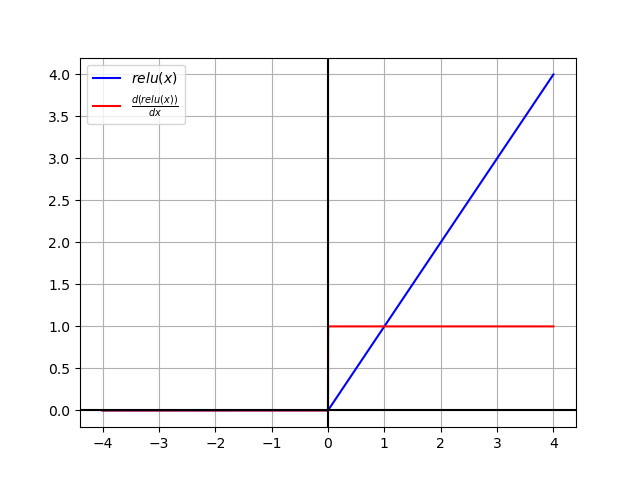
\includegraphics[width=0.5\textwidth]{Images/relu.png}
    \centering
    \caption{ReLU function with its derivative}
    \label{relu graph}
    \end{figure}

    
    \paragraph{Sigmoid function}
    
    \begin{equation}
    \label{def: sigmoid}
        \sigma: \mathbb{R} \mapsto (0,1); \; \; \; \; \sigma(x)=\frac{1}{1+e^{-x}}, 
    \end{equation}
    
    \par Sigmoid is used as output for Bernoulli distribution, or binary classification problems. It maps to an interval $(0,1)$ so the output could be interpreted as the probability of a sample belonging to a selected category. For very positive and very negative values sigmoid saturates, meaning its derivative is close to 0 and the learning is stabilized. This effect can negatively influence learning if used as an activation of hidden layers. Thus sigmoid is used on the output layer or in recurrent neural networks
    
    \begin{figure}[h]
    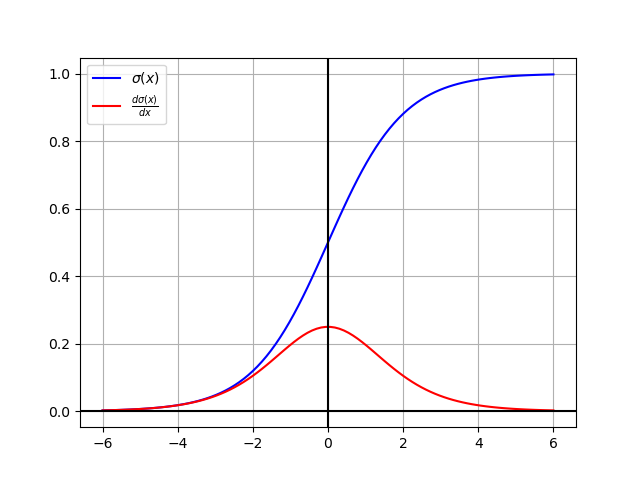
\includegraphics[width=0.5\textwidth]{Images/sigmoid.png}
    \centering
    \caption{Sigmoid activation function with its derivative}
    \label{sigmoid graph}
    \end{figure}

    
    \paragraph{Hyperbolic tangent}
    \begin{equation}
    \label{def: tanh}
        tanh: \mathbb{R} \mapsto (-1,1); \; \; \; \; tanh(x)=\frac{e^x - e^{-x}}{e^x + e^{-x}}, 
    \end{equation}
    Tangent as well a subject to saturation. 
    \begin{figure}[h]
    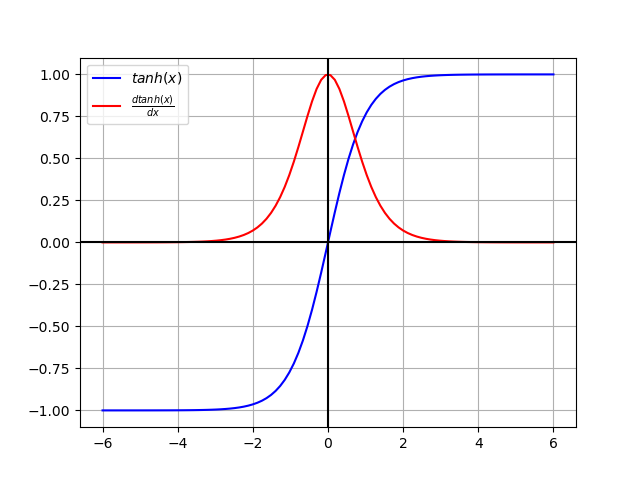
\includegraphics[width=0.5\textwidth]{Images/tanh.png}
    \centering
    \caption{Hyperbolic tangent}
    \label{tanh graph}
    \end{figure}

\section{Loss functions}
To evaluate the performance of our model, we need to describe a function that measures the quality of our outputs made by the neural network with respect to the correct label. Generally, in optimization problems, this function is called the objective function. 


















\section{Convolutional neural network}


Another core architecture of deep learning is a convolutional neural network. Unlike densely connected feed-forward networks, they have sparse connections between individual layers. CNNs are suited for grid-like data structures such as pixel grids of pictures or taking samples at regular time intervals, e.g. time series. Convolution for functions $f$ and $g$ is defined as:

\begin{equation}
    (f*g)(x) = \int_{\mathbb{R}^n} f(x-y)g(x)dy
\end{equation}

We can think of convolution intuitively as a weighted average (the weight is $f$) of all translations of a function $g$. In a computer, we can store information only discretely, e.g. pixels, information at a specific time, or a video that is composed of multiple pictures. Therefore, the values of both functions are discretized, changing the integral into a weighted sum.

\begin{equation}
    (f*g)(t) = \sum_{m= -\infty}^{\infty} f(t-m)g(t)
\end{equation}

The convolution operation differs slightly from a convolution in terms of neural networks. The real operation we will be using is, in fact, the cross-correlation.

\begin{equation}
    (f \star g)(t) = \sum_{m = -\infty}^{\infty} f(t+m)g(t)
\end{equation}

The difference between cross-correlation and convolution is that, in convolution operation, one of the signals is flipped before sliding it over the other. This flipping of a signal provides commutativity for the convolution, which is not as important when it comes to neural network implementation, and also, the cross-correlation operation is much easier to visualize and understand intuitively. To keep the convention of the deep learning community, we will refer to the cross-correlation operation as a convolution, while maintaining the sign $\star$. To functions $f$ and $g$ is often referred to as the input $I$, resp. kernel or a filter $K$. For example, convolution applied on the two-dimensional image's pixel grid would be: 

\begin{equation}
    (I \star K)(i,j) = \sum_m\sum_n I(i+m,j+n)K(m,n)
\end{equation}

Other way thinking about convolutional layers is that they are fully connected layers with shared parameters and sparse interactions between layers. Sparse interactions of the convolutional layer achieve less parameters to learn for training. This means we need to store fewer parameters, which improves the memory requirements of a model. Number of parameters remain constant Sparse interactions provide the ability to describe different, sometimes complicated features efficiently, which would be if learned by densely connected layers, rather difficult.  Parameter sharing meaning instead of learning multiple parameters for the kernel for every location, we only learn one set. 

From an implementation point of view, we need to specify a few more things to complete convolution operation, stride and padding:
\par The stride is denoting that every output pixel is c 









\section{Recurrent neural networks}
Family of networks for processing sequential data. 












\section{Gradient descent}

Optimization refers to the minimization of a loss function. In neural networks, the loss function is generally a non-convex function that depends on tens of thousands, or possibly millions, of variables. Therefore, the analytical approach to find a minimum of our loss function is in most cases computationally very demanding, so a numerical method is needed. 
\par Gradient descent is an iterative optimization method used across the whole field of machine learning. The gradient of a function $f$: $\mathbb{R}^n \mapsto \mathbb{R}$ is a $n$-dimensional row vector, where its components are partial derivatives of the function: 
$$\nabla f(\Vec{x}) := (\frac{\partial f}{\partial x_1}(\Vec{x}), \frac{\partial f}{\partial x_2}(\Vec{x}), \dots, \frac{\partial f}{\partial x_n}(\Vec{x}))$$ 
Gradient $\nabla f(\Vec{a})$ could be geometrically represented as the direction of the steepest ascend. This outcome of multi-variable calculus gives us another way of finding a minimum of a function. Let $x \in \mathbb{R}^n$ be our given starting point and we want our algorithm to propose a new point $\Vec{x}$, such as $\Vec{x}', \; f(\Vec{x'}) \le f(\Vec{x})$. 

\begin{equation}
    \label{vanila gradient descent}
    \Vec{x'} = \Vec{x} - \epsilon \nabla f(\Vec{x})
\end{equation}

The $\epsilon$ stands for a learning rate that defines how big a step we want to take in the direction of a $\nabla f(\Vec{x})$. But usually our data set contains multiple data points and we want our classifier to make the best prediction in expected value over the whole data set or batch. 

\begin{equation}
    \label{BGD}
   E(\theta) = \mathbb{E}_{(\Vec{x}, y) \sim p_{data}} L(f(\Vec{x}, y;\Theta ) = \frac{1}{m} \sum_{i=1}^m L ( \Vec{x^{(i)}}, y^{(i)},  \Vec{\Theta} )
\end{equation}

Then the algorithm changes to:
$$
\Vec{\theta_{n+1}} = \Vec{\theta_{n}} - \epsilon \nabla E(\Vec{\theta_{n}})
$$
The convergence of gradient descent is not automatically guaranteed. We can set conditions under which this method converges.  In practice, the algorithm often finds a sufficiently low loss function value. 
\par We can estimate a gradient and possibly speed up the calculation. For example, using a singular example is an unbiased estimate of our $E(\theta)$. This method is called \textbf{Stochastic Gradient Descent}. Choosing only one example per step is a very noisy estimator, so the standard technique is to do mini-batches. That is, select $m'$ random independent examples from the data to form a batch and compute the gradient only for those examples. 

\begin{equation}
    \label{SGD}
   E(\theta) \approx \frac{1}{m} \sum_{i=1}^{m'} L ( \Vec{x^{(i)}}, y^{(i)},  \Vec{\Theta} ) 
\end{equation}

\subsection{Optimizers}
Optimizers serve as a performance booster for training algorithms. Instead of doing the same step every time, we adjust the learning rate using different techniques such as momentum or adapting it based on the magnitude of a gradient. In this section appears a new operation $\xleftarrow{}$

\paragraph{SGD with momentum}
\paragraph{SGD with Nestorov momentum}
\paragraph{Adagrad}
\subsection{Optimizers with adaptive learning rates}
\paragraph{RMSProp}
\paragraph{Adam}
\paragraph{AdamW}
\section{Back-propagation}
Neural network is a composition of multiple functions, hence calculating the gradient for it to learn would mean finding a derivative of a composite function. The chain rule of calculus states, that for functions $f: \Omega \subset \mathbb{R}^n \mapsto \mathbb{R}^m$ and $g: U \subset \mathbb{R}^m \mapsto \mathbb{R}^p$, where $U \subset f(\Omega)$ $f$ is differentiable at $a \in \Omega$ and  $g$ is differentiable at  $f(a)$. 

\begin{equation}
    \frac{\partial(g \circ f)_k}{\partial x_i}(a) = \sum_{j=1}^{m} \frac{\partial g_k}{\partial y_j}(f(a))\frac{\partial f_j}{x_i}(a)
\end{equation}

This formula suggests us to calculate the gradient from the last layer to the first because the output of the layer $k$-the layer is explicitly dependent only on outputs from $(k-1)$-th layer. Let's remark, that backpropagation is not only chain rule, but the implementation is as important since we want to store previously calculated derivatives and use them in further calculations. Our goal is to calculate the gradient of a loss function with respect to all trainable weights. Let first denote operation in $k$-th layer: 
\begin{equation}
    y^k = f^k(\Vec{W}^k + \Vec{y}^{k-1} + b^k
\end{equation}

where $k \in \widehat{n}$ and $\Vec{W}$ is a weight matrix. 
\begin{equation}
    \frac{\partial L}{\Vec{y}} 
\end{equation}

\begin{equation}
    \frac{\partial L}{\Vec{y}^{n}} = \frac{\partial L}{\Vec{y}\frac{\partial \Vec{y}}{\partial \Vec{y}^{n}} =  
\end{equation}


\section{Regularization}
Weight decay, Early stopping, 






















\section{Weight initialization}
Before beginning training of the NN, weight initialization is necessary. If weights are set to a constant number, it could cause a symmetry problem. During backpropagation, all neurons in the same layer will have the same gradient and would be updated in the same direction. To prevent this problem, weights need to be initialized randomly. Normal approach is to select them form either uniform or normal distribution. Prior to 2010, weights were initialized as follows: 
$$
W_{i,j} \backsim \mathcal{U}\left[\,-\frac{1}{\sqrt{n_i}}, \frac{1}{\sqrt{n_i}}\, \right]
$$
Where $n_i$ is a number of inputs in i-th layer. 
\subsection{Xavier Glorot's initialization}
Study of Xavier Glorot and Yoshua Bengio showed, that weights are not updated equally across the whole network, i.e., gradient of the first layer is significant. This phenomenon negatively effects the learning process.

\begin{equation}
\label{}
     W_{i,j} \backsim \mathcal{U}\left[\,-\sqrt{\frac{6}{n_i+m_i}}, \sqrt{\frac{6}{n_i+m_i}}\, \right]
\end{equation}
       

\subsection{Kaiming He's classification}
\begin{equation}
\label{kaiming he init}
    W_{i,j} \backsim \mathcal{U}\left[\,-\sqrt{\frac{6}{n_i}}, \sqrt{\frac{6}{n_i}}\, \right], \; \;\;
    W_{i,j} \backsim \mathcal{N}\left[\, O , \sqrt{\frac{6}{n_i}}\, \right]
\end{equation}
\bibliography{bibliography}


\chapter{Time series classification architectures}
\section{History}
\label{sec:History}

Neurons serve as the fundamental units of the nervous system, facilitating the transportation of information between the external world, our muscles and brain. The initial concept of creating an artificial neuron capable of imitating real neuron behaviour was proposed by Warren McCulloch and Walter Pitts in 1943. The most basic neural network known today was presented by M. Minsky and S. Papert in 1969. It consisted of a single layer and used a non-linear activation function for the output. However, they received significant criticism as the perceptron is working as linear binary classifier and is unable to learn the XOR function. This shortcoming was one of the factors behind the decline in interest in the development of artificial intelligence, a period known as the AI winter. 


\chapter{Numerical experiments}


\pagestyle{headings}
\bibliographystyle{plain}
\bibliography{bibliography}
\end{document}
